\begin{frame}{Simple Photoemission from a Metal}
  \begin{center}
  \begin{tikzpicture}[every node/.style={transform shape}]
    \node (electron) [circle,fill=pink,draw,label=above left:{\Large e$^{-}$}] {};
    \fill [blue!50] 
      ($(electron) + (-2cm,-3cm)$) node [left,black] {\Large $\varepsilon_{\scriptscriptstyle F} $}
      -- ++(+2cm,0) node (surface) {}
      -- ++(0,-2cm) node (sub-surface) {}
      -- ++(-2cm,0);
    
    \draw [gray,line width=2mm,->,>=latex']
      (surface.center) 
      -- (electron) node [midway] (photon) {};
    
    \draw [line width=1.5mm,<-,>=latex,decorate,blue,decoration={snake,pre=lineto,pre length=7mm}]
      (photon)
      -- ++(-2cm,0) node [midway,above=3mm,black] {\large $ \hbar \omega $};
      
    \draw [gray,line width=0.5mm] 
      (surface) ++(1cm,0) -- ++(3cm,0) node [pos=0.3] (x-phi) {};
  
    \draw [line width=0.7mm,dashed]
      (surface.center) to [out=80,in=180] ($(electron -| x-phi) + (0,5mm)$) -- ++(2cm,0) node [label=above right:{$ E_{DC}=0 $}] (upper-no-field) {};
    \draw [line width=0.7mm]
      (sub-surface.center) -- (surface.center) to [out=80,in=160] ($(electron -| x-phi) - (0,4mm)$) node (upper) {} -- ++(-20:2.2cm);
  
    \draw [line width=1mm,->,>=latex,pink] 
      (electron) -- ++(5cm,0) 
        node (exit) {}
        node [right,black] {$\Delta p_{\smallT} = \sqrt{\frac{m (\hbar \omega - \Phi_{eff})}{3}}$};
    \node [below=of exit,shape=single arrow,minimum height=1cm,draw,fill=red,label={[yshift=-5mm]below:{$ E_{DC} $}},rotate=180] {};
    
    \draw [<->,>=latex] (x-phi) -- (upper) node [pos=0.4,right] {\large $ \Phi_{eff} < \Phi $};
    \draw [<->,>=latex] (upper-no-field) -- (upper-no-field |- surface.north);

    \node<2-> [red] at (4cm,-4cm) {$\eta_{PE} = A (1-R) (\hbar \omega - \Phi_{eff})^2$};
  \end{tikzpicture}
  \end{center}
\end{frame}

\begin{frame}{Driving a Plasmon (Back-Illuminated)}
  \begin{columns}
  \begin{column}{0.54\linewidth}
    \begin{center}
    \begin{tikzpicture}
      \filldraw [fill=gray!10]
      (0,0)
      node [below left] {Glass}
      rectangle (-2,-5)
      ;
      \filldraw
        [fill=orange]
        (0,0) 
        node [name=photocathode1,above right]{Au Film ($\varepsilon$)}
        -- ++(0.2,0)
        -- ++(0,-5)
        node [name=source,midway] {} 
        -- ++(-0.2,0)
        -- (0,0)
        node [name=laser,midway] {}
        -- cycle
      ;
      \draw
        [-latex,ultra thick,green] 
        ($(laser) + (-135:3.5)$) 
        -- (laser.west)
        node [left=0.3,name=laser label,pos=0.8,black,fill=white] {Laser ($\lambda$)}
      ;
      \fill
        [blue!30]
        (source.center)
        -- ++(3,2mm)
        -- ++(0,-4mm)
        -- cycle
      ;
      \draw
        [-latex,ultra thick,blue]
        (source.center)
        -- ++(3,2mm)
      ;
      \draw
        [-latex,ultra thick,blue]
        (source.center)
        -- ++(3,-2mm)
        node [name=electron label,pos=0.5,black,below=0.2,align=center]{Photoemitted\\Electrons}
      ;
      \draw
        [dashed]
        (source)
        -- ++(3.3,0)
      ;
      \draw 
        ($(laser) + (0,-1)$) 
        arc (-90:-135:1)
        node [below=0.3] {$\theta$}
      ;
    \end{tikzpicture}
    \end{center}
  \end{column}
  \begin{column}{0.44\linewidth}
    \begin{figure}
      \centering
      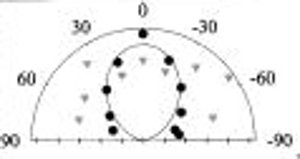
\includegraphics[scale=0.8]{plasmon_reduction_angle}
      \caption{The measured angular distribution of photoelectrons
in the plane of incidence (dots) and perpendicular to that (triangles), as
well as a fit to a $\cos^2\theta$ distribution.\footcite{zawadzka_evanescent}}
    \end{figure}
  \end{column}
  \end{columns}
\end{frame}

\begin{frame}{Driving a Plasmon (Front-Illuminated)}
  \begin{columns}
    \begin{column}{0.49\linewidth}
  \begin{center}
  \begin{tikzpicture}
    \filldraw
      [fill=orange]
      (0,0) 
      node [name=photocathode1,below right]{Au}
      node [below=1mm of photocathode1] {$\varepsilon$}
      -- ++(1,0)
      decorate [decoration=snake,segment length=5mm]{ 
        -- ++(0,-5)
        node [name=source,midway] {} 
      } 
      -- ++(-1,0)
      -- cycle
    ;
    \draw [|-|]
      ($(source) + (-4mm,-14mm)$)
      -- ++(0,-5mm)
      node [midway,left] {$a$}
    ;
    \begin{pgfonlayer}{background}
      \foreach \x in {8.5mm,3.5mm,-1.5mm,-6.5mm} {
        \fill<2->
          [fill=red]
          ($(source) + (0,\x)$) 
          ellipse (6mm and 2.5mm)
        ;
        \fill<2->
          [fill=red!50]
          ($(source) + (0,\x)$)
          ellipse (3mm and 1.5mm)
        ;
      }
    \end{pgfonlayer}
    \draw
      [-latex,ultra thick,green] 
      ($(source) + (45:3.5)$) 
      -- (source.east)
      node [name=laser label,pos=0.3,black,fill=white] {Laser ($\lambda$)}
    ;
    \fill<3->
      [blue!30]
      (source.east)
      -- ++(3,2mm)
      -- ++(0,-4mm)
      -- cycle
    ;
    \draw<3->
      [-latex,ultra thick,blue]
      (source.east)
      -- ++(3,2mm)
    ;
    \draw<3->
      [-latex,ultra thick,blue]
      (source.east)
      -- ++(3,-2mm)
      node [name=electron label,pos=0.8,black,above=0.5,align=center]{Photoemitted\\Electrons}
    ;
    \draw
      [dashed]
      (source)
      -- ++(4,0)
    ;
    \draw 
      ($(source) + (1,0)$) 
      arc (0:41:1)
      node [right=0.3] {$\theta$}
    ;
    \node<2-> [anchor=west,align=center] at ($(source) + (0.3,-1.2)$) {Plasmon\\Oscillation};
  \end{tikzpicture}
  \end{center}
    \end{column}
    \begin{column}{0.49\linewidth}
      To drive a surface plasmon by front-illumination align so that:
      \begin{align*}
        k_{SP} =& k_{laser}^{\parallel} + k_{G}\\
        \sin(\theta) =& \sqrt{ \frac{\varepsilon}{1+\varepsilon} } - \frac{\lambda}{a}
      \end{align*}
      where $\varepsilon$ is the metal's dielectric constant
      \begin{block}<4->{Why Gold?}
        Surface plasmon frequency is near 2nd harmonic (green) of our Yb:KGW laser
      \end{block}
    \end{column}
  \end{columns}
\end{frame}

\begin{frame}{First Attempt (Gold on Glass)}
  \begin{columns}
    \begin{column}{0.49\linewidth}
      First attempt:
      \begin{itemize}
        \item Commercial optical grating
        \item Gold on glass substrate
        \item 750 lines per mm
      \end{itemize}
      \visible<2->{
        \begin{block}{Result}
          Insufficient heat conduction though glass substrate
        \end{block}
      }
    \end{column}
    \begin{column}{0.49\linewidth}
      \begin{figure}
        \centering
        \visible<2->{
          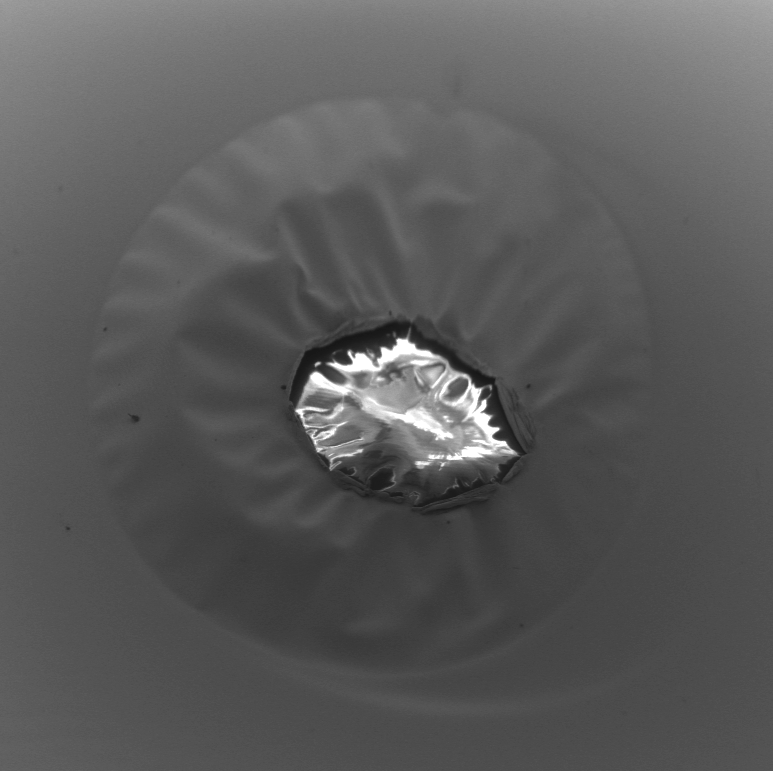
\includegraphics[width=0.8\linewidth]{Damage}
        }
      \end{figure}
    \end{column}
  \end{columns}
\end{frame}

\begin{frame}{Second attempt (Gold on FIB milled silicon)}
  To avoid heat problems:
  \begin{itemize}
    \item Silicon substrate
    \begin{itemize}
      \item Focused Ion Beam (FIB) milled at Argonne Nat'l Lab (ANL)
      \item Near sinusoidal shape
      \item $\sim 1 \mu$m periodicity
      \item Several ($\sim10$) 100$\mu$m x 100$\mu$m patches
      \item Several hours of milling
    \end{itemize}
    \item Gold coated at UIC Nano Core Facility (NCF)
    \begin{itemize}
      \item 300 nm thickness
      \item Chromium binding layer
    \end{itemize}
  \end{itemize}
  
\end{frame}

\begin{frame}{Sinusoidal Nanopatterned Photocathode}
  \begin{tikzpicture}
    \begin{pgfonlayer}{below-main}
      \node[name=low,label=below:Low Mag]{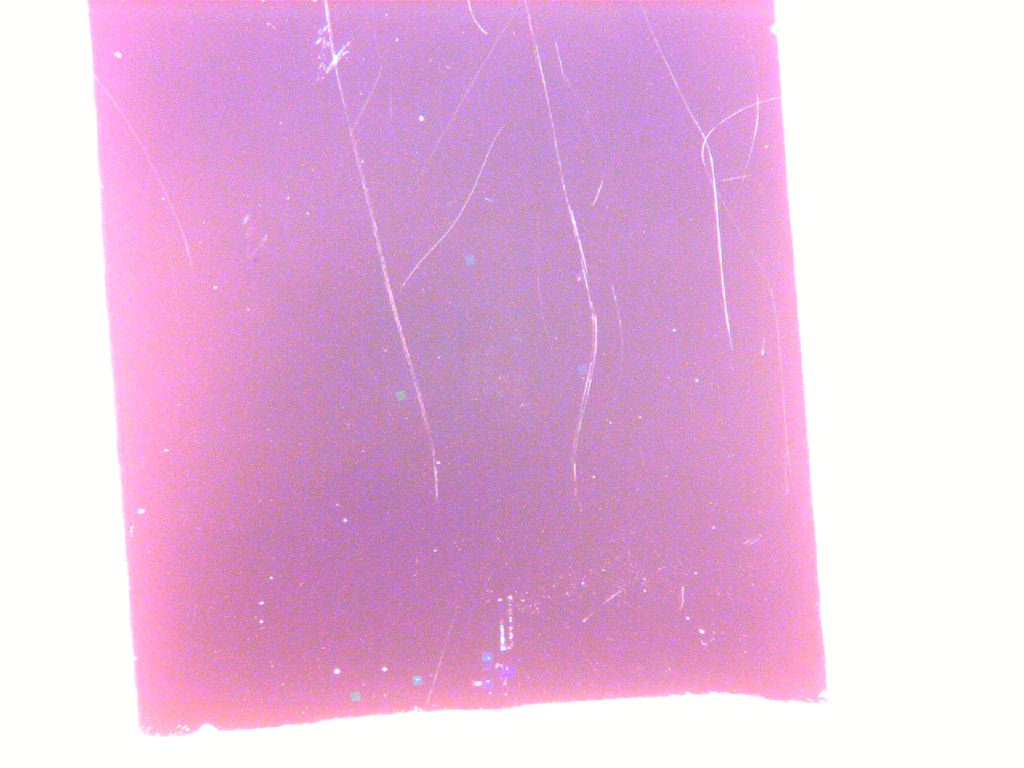
\includegraphics[width=2in]{FIB-low}};
    \end{pgfonlayer}
    \draw<2->
      (-7mm,8mm) node [name=low-top-left] {}
      -- ++(12mm,0) node [name=low-top-right] {}
      -- ++(0,-10mm) node [name= low-bottom-right] {}
      -- ++(-12mm,0) node [name= low-bottom-left] {}
      -- cycle
    ;
    \visible<3->{
      \node [
        inner sep=0,
        right=8mm of low.center,
        yshift=2.3cm,
        name=medium,
        label=above:Medium Mag
      ] {
        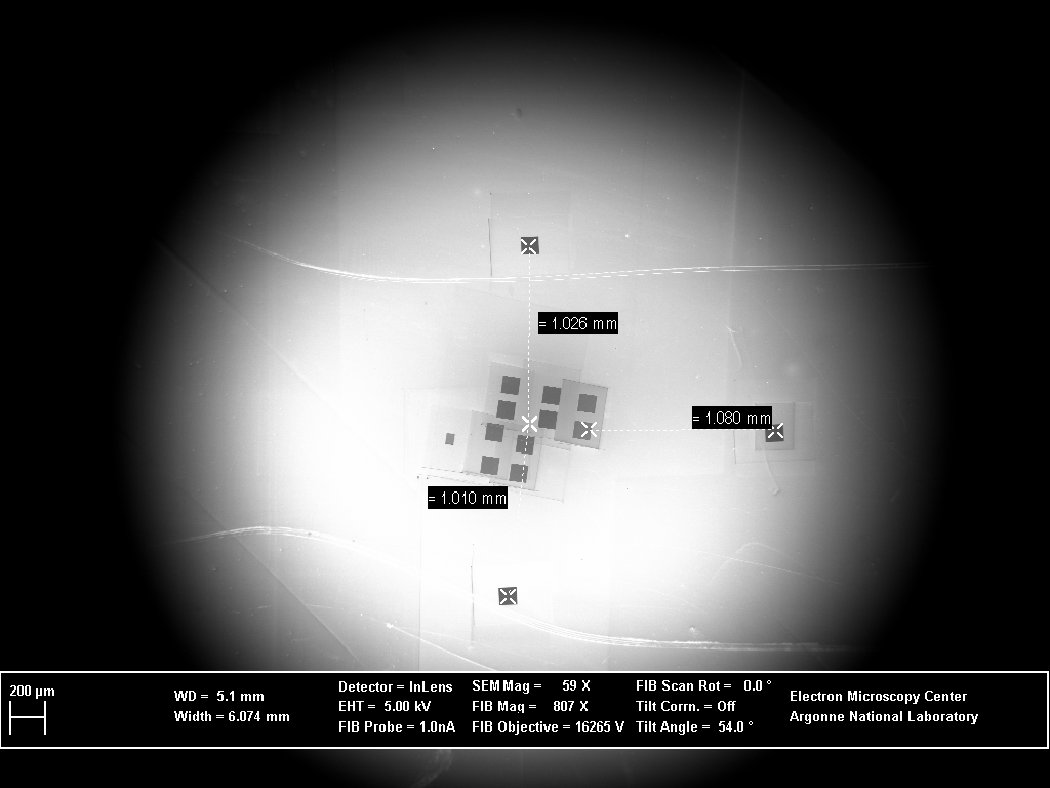
\includegraphics[width=2in]{FIB-medium}
      }
      ;
    }
    \begin{pgfonlayer}{below-main}
      \draw<3-> (low-top-left.center) -- (medium.north west);
      \draw<3-> (low-top-right.center) -- (medium.north east);
      \draw<3-> (low-bottom-left.center) -- (medium.south west);
      \draw<3-> (low-bottom-right.center) -- (medium.south east);
    \end{pgfonlayer}
    \begin{pgfonlayer}{above-main}
      \visible<5->{
        \node [
          inner sep=0,
          name=high,
          below right=1cm of medium.center,
          label=below:High Mag
        ] {
          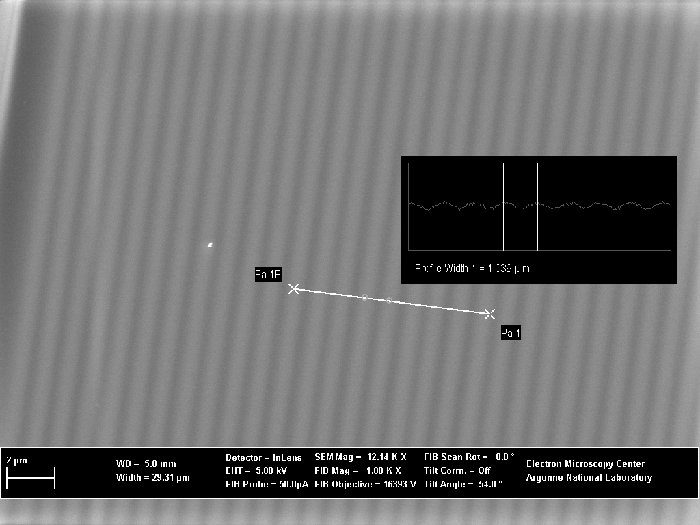
\includegraphics[width=2in]{FIB-high}
        };
      }
    \end{pgfonlayer}
    \node [name=feature, right=2.3mm of medium.center,inner sep=0.7mm,yshift=-0.5mm] {};
    \draw<4->
      (feature.north east)
      -- (feature.north west)
      -- (feature.south west)
      -- (feature.south east)
      -- cycle
    ;
    \draw<5-> (feature.north east) -- (high.north east);
    \draw<5-> (feature.north west) -- (high.north west);
    \draw<5-> (feature.south east) -- (high.south east);
    \draw<5-> (feature.south west) -- (high.south west);
  \end{tikzpicture}
\end{frame}

\begin{frame}{Sinusoidal Nanopatterned Photocathode: Results}
  \begin{center}
    \begin{tikzpicture}
      \node {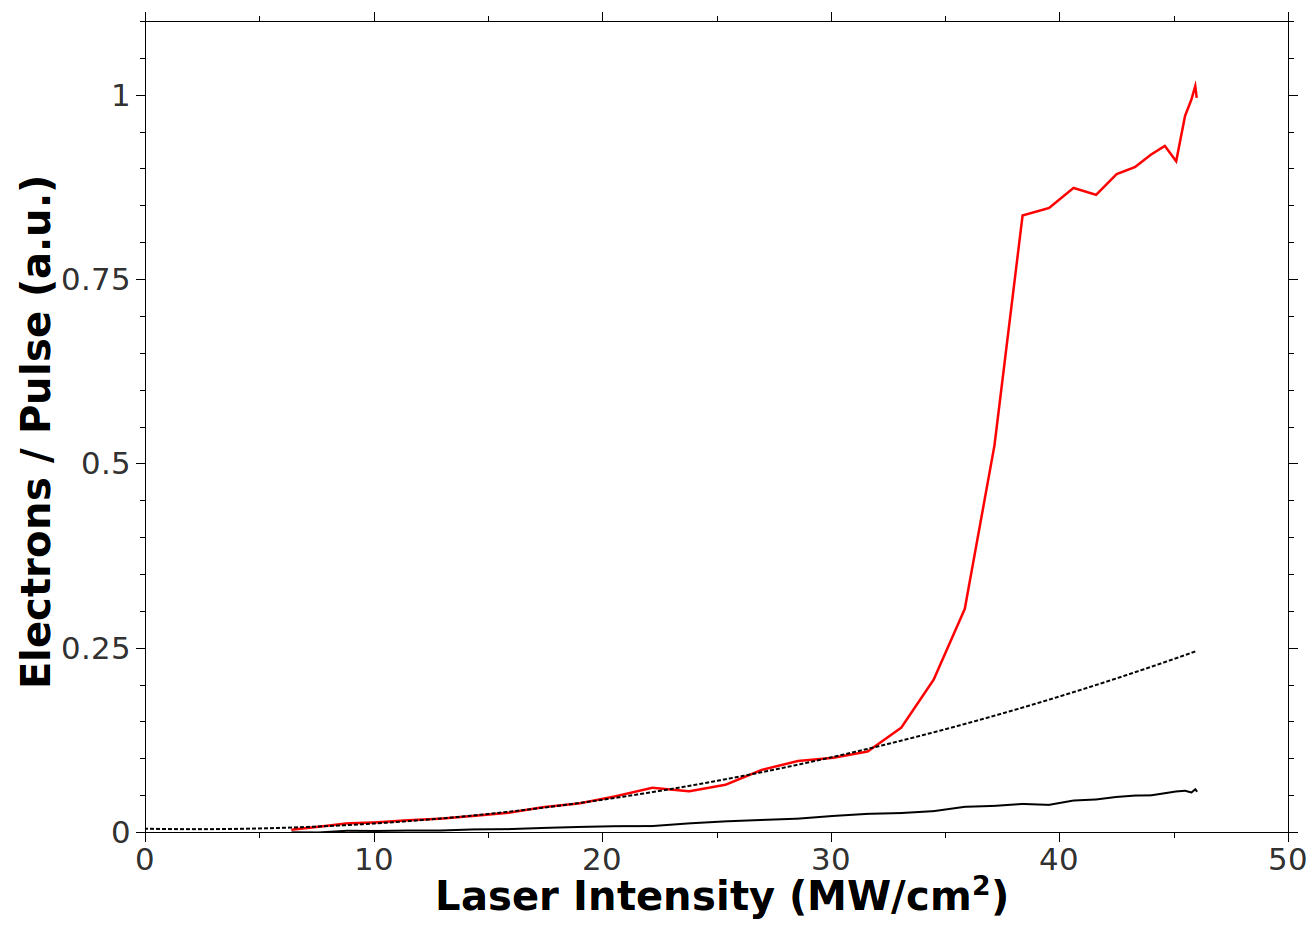
\includegraphics{Graph1}};
      \node<2> at (-1.8,1.8) [draw] {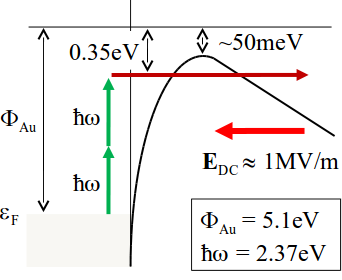
\includegraphics[width=1.2in]{PE_diag_0}};
      \node<3> at (-1.8,1.8) [draw] {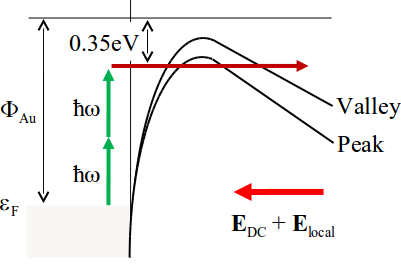
\includegraphics[width=1.2in]{PE_diag_1}};
      \node<4> at (-1.8,1.8) [draw] {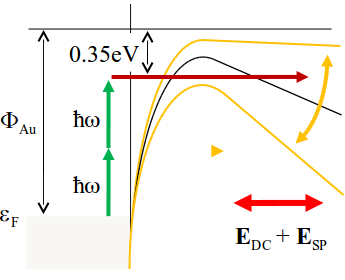
\includegraphics[width=1.2in]{PE_diag_2}};
      
      \node<1,3-4> at (2.1,2.8) [red,align=right] {Plasmon Enhanced\\Photoemission};
      \node<1> at (3.5,-0.7) {Fit $I^2$};
      
      \node<1-2> at (-1,-1.5) (TwoPhoton Label) [align=left] {Two Photon\\Photoemission};
      \draw<1-2> [thick,-latex]
        (TwoPhoton Label)
        to [out=0,in=110] (2.7,-2.2)
      ;
      
      \node<2> 
        at (3,1.7) 
        [label={below:Isotropic $\Delta p_{\scriptscriptstyle T}$}] 
        {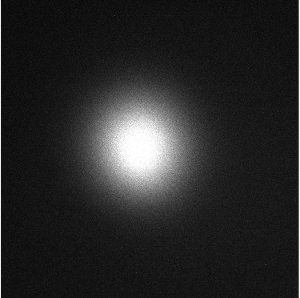
\includegraphics[width=1in]{final-fourier-2photon-036}}
      ;
      
      \node<3> 
        (fourier image)
        at (-2,-1) 
        [
          shape=rectangle callout, callout relative pointer={(0.9,-0.5)}, 
          draw, fill=white
        ] 
        {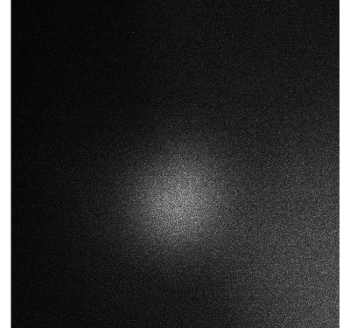
\includegraphics[width=1in]{final-fourier-022}}
      ;
      \node<3> [right=0.2 of fourier image] {Isotropic $\Delta p_{\scriptscriptstyle T}$};
      
      \node<4>
        at (-1.5,-1)
        [
          shape=rectangle callout, callout relative pointer={(1,-0.2)}, 
          draw, fill=white, align=left
        ] 
        {Onset of barrier suppression\\$\Rightarrow E_{SP} \approx$ 40MV/m}
      ;
      
      \node<5-> 
        at (-1.8,-1.4)
        [
          shape=rectangle callout, callout relative pointer={(1.9,-0.45)}, 
          draw, fill=white, align=left
        ] 
        {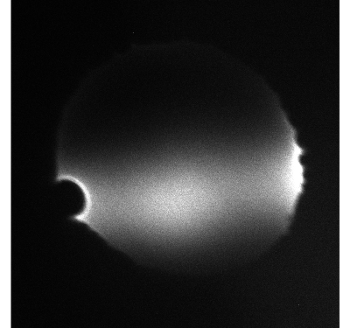
\includegraphics[width=0.7in]{final-fourier-026}}
      ;
      \node<5-> 
        at (0.5,0)
        [
          shape=rectangle callout, callout relative pointer={(0.7,-0.4)}, 
          draw, fill=white, align=left
        ] 
        {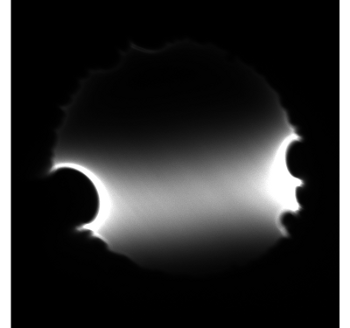
\includegraphics[width=0.7in]{final-fourier-030}}
      ;
      \node<5-> 
        at (1.2,2.2)
        [
          shape=rectangle callout, callout relative pointer={(1,0)}, 
          draw, fill=white, align=left
        ] 
        {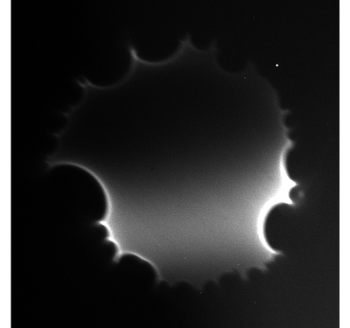
\includegraphics[width=0.7in]{final-fourier-038}}
      ;
      \node<5->
        at (-2,1.8)
        {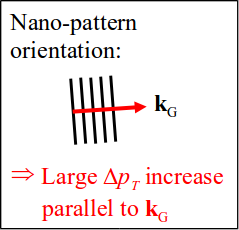
\includegraphics[width=1in]{PE_diag_3}}
      ;
    \end{tikzpicture}
  \end{center}
\end{frame}

\begin{frame}{Understanding Observed $\Delta p_{\scriptscriptstyle T}$ Increase}
  Is the 1D broadening due to the plasmon or the surface?
  \begin{center}
    \begin{tikzpicture}
  \draw [thick,->,green] 
    (0,0) -- ++(3,0) 
      node [pos=0.5,below,black,align=center] {$k_L \sin \theta$\\$\theta \approx 39^{\circ}$}
  ;
  \draw [thick,->,red]
    (3,0) -- ++(2,0)
      node [pos=0.5,below,black] {$k_G$}
  ;
  \draw [thick,->,blue]
    (0,0.2) -- ++(5,0)
      node [pos=0.5,black,above] {$k_{SP}$}
  ;
  \node at (7,0) {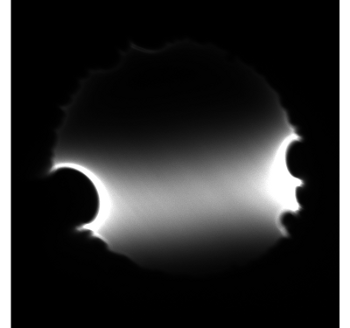
\includegraphics{final-fourier-030.png}};
  \draw [very thick,red] (6,-0.4) -- ++(9:2.2);

  \draw [thick,->,green] 
    (0,-3.5) -- ++(3,0) 
      node [pos=0.5,below,black,align=center] {$k_L \sin \theta$\\$\theta \approx 47^{\circ}$}
  ;
  \draw [thick,dashed,green] 
    (3,-3.5) -- (4,-3.5)
      node [above,black,pos=0.8] {$45^{\circ}$}
  ;
  \draw [thick,->,red]
    (3,-3.5) -- ++(1.4,1.4)
      node [pos=0.4,left,black] {$k_G$}
      coordinate [pos=1] (end)
  ;
  \draw [thick,->,blue]
    (0,-3.5) -- (end)
      node [pos=0.5,black,above] {$k_{SP}$}
  ;
  \node at (7,-3) {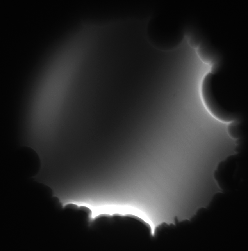
\includegraphics{rotated.png}};
  \draw [very thick,green,dashed] 
    (6,-2.7) -- ++(9:2.2)
      node [pos=0.7,below, white] {$45^{\circ}$}
      coordinate [pos=1] (rotate end)
  ;
  \draw [very thick,red]
    (rotate end) -- ++(234:2.2)
  ;
\end{tikzpicture}

  \end{center}
\end{frame}

\begin{frame}{Trenched Nanopatterned Photocathode}
  \begin{columns}
    \begin{column}{0.54\linewidth}
      Grooved Photocathode
      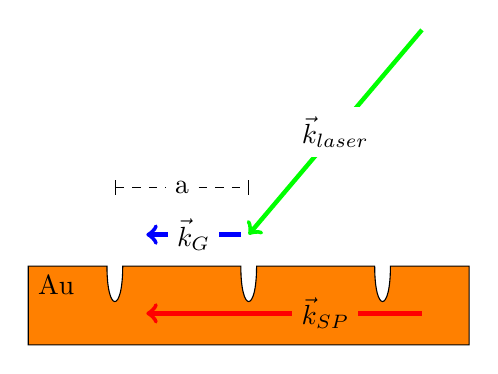
\begin{tikzpicture}
        \draw 
          [fill=orange]
          (0,0)
            node [below right] {Au}
          -- (1,0)
            .. controls (1,-0.6) and (1.2,-0.6)
          .. (1.2,0)
          -- (2.7,0)
            .. controls (2.7,-0.6) and (2.9,-0.6)
          .. (2.9,0)
          -- (4.4,0)
            .. controls (4.4,-0.6) and (4.6,-0.6)
          .. (4.6,0)
          -- (5.6,0)
          -- (5.6,-1)
          -- (0,-1)
          -- cycle
        ;  
        \draw [|-|,dashed]
          (1.1,1)
          -- (2.8,1)
            node [pos=0.5,fill=white] {a}
        ;
    
        \draw [ultra thick,red,->]
          (5,-0.6)
          -- (1.5,-0.6)
            node [pos=0.35,black,fill=orange] {$\vec{k}_{SP}$}
        ;
        \draw [ultra thick,green,->]
          (5,3)
          -- (2.8,0.4)
            node [pos=0.5,black,fill=white] {$\vec{k}_{laser}$}
        ;
        \draw [ultra thick, blue, ->]
          (2.7,0.4)
          -- (1.5,0.4)
            node [pos=0.5,black,fill=white] {$\vec{k}_{G}$}
        ;
      \end{tikzpicture}
    \end{column}
    \begin{column}{0.44\linewidth}
      \begin{align*}
        k_{SP} =& k_{laser}^{\parallel} + m \cdot k_{G}\\
        \sin(\theta) =& \sqrt{ \frac{\varepsilon}{1+\varepsilon} } - \frac{ m \lambda }{a}
      \end{align*}
      \begin{block}<2->{}
        \begin{itemize}
          \item Retains periodic structure
          \item Reduced $\nabla_{\perp} E_{SP}$
          \item Additional Fourier components
          \item Easier to FIB mill
        \end{itemize}
      \end{block}
    \end{column}
  \end{columns}
\end{frame}

\begin{frame}{Trenched Nanopatterned Photocathode: Results}
  \begin{columns}
    \begin{column}{0.49\linewidth}
      \begin{figure}
        \centering
        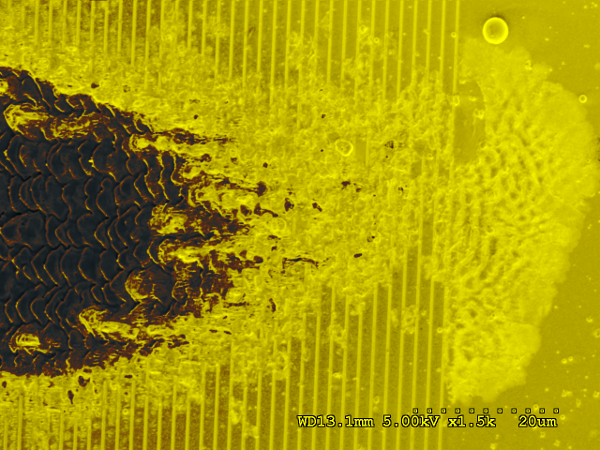
\includegraphics{trench_damage_false_color.png}
      \end{figure}
      \begin{itemize}
        \item Heat damage on grating
        \item Plasmon excitation?
      \end{itemize}
    \end{column}
    \begin{column}{0.49\linewidth}
      \begin{figure}
        \centering
        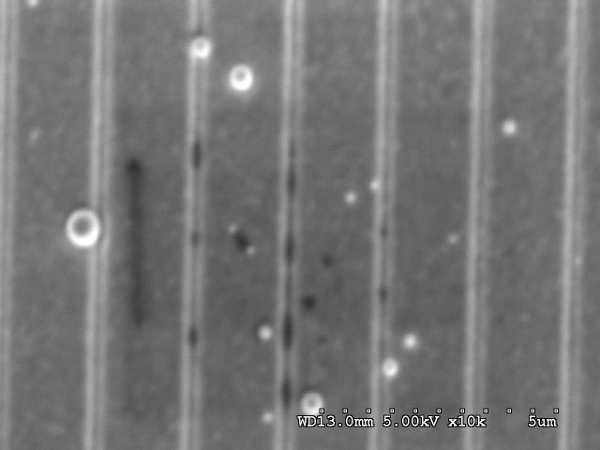
\includegraphics{trench_incomplete_filling.png}
      \end{figure}
      \begin{itemize}
        \item Incomplete filling of trenches
        \item Increases plasmon threshold 
        \item[$\Rightarrow$] laser damage 
      \end{itemize}
    \end{column}
  \end{columns}
  \vfill
  \begin{center}
    \alert{No evidence of plasmon-assisted photoemission!}
  \end{center}
\end{frame}

\begin{frame}{III-Antimonide Photocathodes}
  \begin{columns}
    \begin{column}{0.30\linewidth}
      \begin{itemize}
        \item No emission expected
        \item<2-> Strong emission observed
        \item<3-> Narrow emission cone angle!
      \end{itemize}
    \end{column}
    \begin{column}{0.68\linewidth}
  \begin{figure}
    \centering
    \visible<2->{
    \begin{tikzpicture}
      \begin{tikzpicture}[gnuplot]
%% generated with GNUPLOT 4.6p0 (Lua 5.1; terminal rev. 99, script rev. 100)
%% Sun 21 Apr 2013 07:00:39 PM CDT
\gpsolidlines
\path (0.000,0.000) rectangle (8.750,6.125);
\gpcolor{color=gp lt color border}
\gpsetlinetype{gp lt border}
\gpsetlinewidth{1.00}
\draw[gp path] (1.688,0.985)--(1.868,0.985);
\draw[gp path] (6.601,0.985)--(6.421,0.985);
\node[gp node right] at (1.504,0.985) { 0};
\draw[gp path] (1.688,1.939)--(1.868,1.939);
\draw[gp path] (6.601,1.939)--(6.421,1.939);
\node[gp node right] at (1.504,1.939) { 200};
\draw[gp path] (1.688,2.893)--(1.868,2.893);
\draw[gp path] (6.601,2.893)--(6.421,2.893);
\node[gp node right] at (1.504,2.893) { 400};
\draw[gp path] (1.688,3.848)--(1.868,3.848);
\draw[gp path] (6.601,3.848)--(6.421,3.848);
\node[gp node right] at (1.504,3.848) { 600};
\draw[gp path] (1.688,4.802)--(1.868,4.802);
\draw[gp path] (6.601,4.802)--(6.421,4.802);
\node[gp node right] at (1.504,4.802) { 800};
\draw[gp path] (1.688,5.756)--(1.868,5.756);
\draw[gp path] (6.601,5.756)--(6.421,5.756);
\node[gp node right] at (1.504,5.756) { 1000};
\draw[gp path] (1.687,0.985)--(1.687,1.165);
\draw[gp path] (1.687,5.756)--(1.687,5.576);
\node[gp node center] at (1.687,0.677) { 0};
\draw[gp path] (2.722,0.985)--(2.722,1.165);
\draw[gp path] (2.722,5.756)--(2.722,5.576);
\node[gp node center] at (2.722,0.677) { 0.04};
\draw[gp path] (3.756,0.985)--(3.756,1.165);
\draw[gp path] (3.756,5.756)--(3.756,5.576);
\node[gp node center] at (3.756,0.677) { 0.08};
\draw[gp path] (4.791,0.985)--(4.791,1.165);
\draw[gp path] (4.791,5.756)--(4.791,5.576);
\node[gp node center] at (4.791,0.677) { 0.12};
\draw[gp path] (5.825,0.985)--(5.825,1.165);
\draw[gp path] (5.825,5.756)--(5.825,5.576);
\node[gp node center] at (5.825,0.677) { 0.16};
\draw[gp path] (6.601,0.985)--(6.421,0.985);
\node[gp node left] at (6.785,0.985) { 0};
\draw[gp path] (6.601,1.939)--(6.421,1.939);
\node[gp node left] at (6.785,1.939) { 500};
\draw[gp path] (6.601,2.893)--(6.421,2.893);
\node[gp node left] at (6.785,2.893) { 1000};
\draw[gp path] (6.601,3.848)--(6.421,3.848);
\node[gp node left] at (6.785,3.848) { 1500};
\draw[gp path] (6.601,4.802)--(6.421,4.802);
\node[gp node left] at (6.785,4.802) { 2000};
\draw[gp path] (6.601,5.756)--(6.421,5.756);
\node[gp node left] at (6.785,5.756) { 2500};
\draw[gp path] (1.688,5.756)--(1.688,0.985)--(6.601,0.985)--(6.601,5.756)--cycle;
\node[gp node center,rotate=-270] at (0.246,3.370) {HWe$^{-1}$M Beam Size ($\mu$m)};
\node[gp node center,rotate=-270] at (8.042,3.370) {Electrons / Pulse};
\node[gp node center] at (4.144,0.215) {UV Laser Pulse Energy (nJ)};
\gpcolor{rgb color={0.000,0.000,0.000}}
\gpsetlinetype{gp lt plot 4}
\draw[gp path] (2.157,4.845)--(2.157,5.370);
\draw[gp path] (2.067,4.845)--(2.247,4.845);
\draw[gp path] (2.067,5.370)--(2.247,5.370);
\draw[gp path] (2.632,4.880)--(2.632,5.393);
\draw[gp path] (2.542,4.880)--(2.722,4.880);
\draw[gp path] (2.542,5.393)--(2.722,5.393);
\draw[gp path] (3.224,4.941)--(3.224,5.386);
\draw[gp path] (3.134,4.941)--(3.314,4.941);
\draw[gp path] (3.134,5.386)--(3.314,5.386);
\draw[gp path] (3.887,5.019)--(3.887,5.427);
\draw[gp path] (3.797,5.019)--(3.977,5.019);
\draw[gp path] (3.797,5.427)--(3.977,5.427);
\draw[gp path] (4.571,5.040)--(4.571,5.367);
\draw[gp path] (4.481,5.040)--(4.661,5.040);
\draw[gp path] (4.481,5.367)--(4.661,5.367);
\draw[gp path] (5.221,4.960)--(5.221,5.338);
\draw[gp path] (5.131,4.960)--(5.311,4.960);
\draw[gp path] (5.131,5.338)--(5.311,5.338);
\draw[gp path] (5.788,5.000)--(5.788,5.424);
\draw[gp path] (5.698,5.000)--(5.878,5.000);
\draw[gp path] (5.698,5.424)--(5.878,5.424);
\draw[gp path] (6.228,4.965)--(6.228,5.462);
\draw[gp path] (6.138,4.965)--(6.318,4.965);
\draw[gp path] (6.138,5.462)--(6.318,5.462);
\draw[gp path] (6.506,5.062)--(6.506,5.458);
\draw[gp path] (6.416,5.062)--(6.596,5.062);
\draw[gp path] (6.416,5.458)--(6.596,5.458);
\draw[gp path] (6.601,5.041)--(6.601,5.467);
\draw[gp path] (6.511,5.041)--(6.691,5.041);
\draw[gp path] (6.511,5.467)--(6.691,5.467);
\gpsetpointsize{4.00}
\gppoint{gp mark 5}{(2.157,5.108)}
\gppoint{gp mark 5}{(2.632,5.137)}
\gppoint{gp mark 5}{(3.224,5.164)}
\gppoint{gp mark 5}{(3.887,5.223)}
\gppoint{gp mark 5}{(4.571,5.203)}
\gppoint{gp mark 5}{(5.221,5.149)}
\gppoint{gp mark 5}{(5.788,5.212)}
\gppoint{gp mark 5}{(6.228,5.213)}
\gppoint{gp mark 5}{(6.506,5.260)}
\gppoint{gp mark 5}{(6.601,5.254)}
\gpcolor{rgb color={0.000,1.000,0.000}}
\gpsetlinetype{gp lt plot 0}
\draw[gp path] (1.688,0.985)--(1.738,1.006)--(1.787,1.028)--(1.837,1.049)--(1.887,1.070)%
  --(1.936,1.091)--(1.986,1.112)--(2.035,1.133)--(2.085,1.154)--(2.135,1.175)--(2.184,1.197)%
  --(2.234,1.218)--(2.284,1.239)--(2.333,1.260)--(2.383,1.281)--(2.432,1.302)--(2.482,1.323)%
  --(2.532,1.344)--(2.581,1.366)--(2.631,1.387)--(2.681,1.408)--(2.730,1.429)--(2.780,1.450)%
  --(2.829,1.471)--(2.879,1.492)--(2.929,1.513)--(2.978,1.535)--(3.028,1.556)--(3.078,1.577)%
  --(3.127,1.598)--(3.177,1.619)--(3.226,1.640)--(3.276,1.661)--(3.326,1.682)--(3.375,1.704)%
  --(3.425,1.725)--(3.475,1.746)--(3.524,1.767)--(3.574,1.788)--(3.623,1.809)--(3.673,1.830)%
  --(3.723,1.851)--(3.772,1.873)--(3.822,1.894)--(3.872,1.915)--(3.921,1.936)--(3.971,1.957)%
  --(4.020,1.978)--(4.070,1.999)--(4.120,2.020)--(4.169,2.042)--(4.219,2.063)--(4.269,2.084)%
  --(4.318,2.105)--(4.368,2.126)--(4.417,2.147)--(4.467,2.168)--(4.517,2.189)--(4.566,2.211)%
  --(4.616,2.232)--(4.666,2.253)--(4.715,2.274)--(4.765,2.295)--(4.814,2.316)--(4.864,2.337)%
  --(4.914,2.358)--(4.963,2.380)--(5.013,2.401)--(5.063,2.422)--(5.112,2.443)--(5.162,2.464)%
  --(5.211,2.485)--(5.261,2.506)--(5.311,2.527)--(5.360,2.549)--(5.410,2.570)--(5.460,2.591)%
  --(5.509,2.612)--(5.559,2.633)--(5.608,2.654)--(5.658,2.675)--(5.708,2.696)--(5.757,2.718)%
  --(5.807,2.739)--(5.857,2.760)--(5.906,2.781)--(5.956,2.802)--(6.005,2.823)--(6.055,2.844)%
  --(6.105,2.865)--(6.154,2.887)--(6.204,2.908)--(6.254,2.929)--(6.303,2.950)--(6.353,2.971)%
  --(6.402,2.992)--(6.452,3.013)--(6.502,3.034)--(6.551,3.056)--(6.601,3.077);
\gpcolor{rgb color={0.000,0.000,0.000}}
\gpsetlinetype{gp lt plot 6}
\draw[gp path] (1.598,0.986)--(1.778,0.986);
\draw[gp path] (1.598,0.986)--(1.778,0.986);
\draw[gp path] (1.704,0.995)--(1.704,0.997);
\draw[gp path] (1.614,0.995)--(1.794,0.995);
\draw[gp path] (1.614,0.997)--(1.794,0.997);
\draw[gp path] (1.784,1.047)--(1.784,1.060);
\draw[gp path] (1.694,1.047)--(1.874,1.047);
\draw[gp path] (1.694,1.060)--(1.874,1.060);
\draw[gp path] (1.995,1.134)--(1.995,1.167);
\draw[gp path] (1.905,1.134)--(2.085,1.134);
\draw[gp path] (1.905,1.167)--(2.085,1.167);
\draw[gp path] (2.393,1.312)--(2.393,1.385);
\draw[gp path] (2.303,1.312)--(2.483,1.312);
\draw[gp path] (2.303,1.385)--(2.483,1.385);
\draw[gp path] (3.003,1.609)--(3.003,1.748);
\draw[gp path] (2.913,1.609)--(3.093,1.609);
\draw[gp path] (2.913,1.748)--(3.093,1.748);
\draw[gp path] (3.792,1.924)--(3.792,2.133);
\draw[gp path] (3.702,1.924)--(3.882,1.924);
\draw[gp path] (3.702,2.133)--(3.882,2.133);
\draw[gp path] (4.674,2.222)--(4.674,2.497);
\draw[gp path] (4.584,2.222)--(4.764,2.222);
\draw[gp path] (4.584,2.497)--(4.764,2.497);
\draw[gp path] (5.519,2.478)--(5.519,2.810);
\draw[gp path] (5.429,2.478)--(5.609,2.478);
\draw[gp path] (5.429,2.810)--(5.609,2.810);
\draw[gp path] (6.185,2.733)--(6.185,3.122);
\draw[gp path] (6.095,2.733)--(6.275,2.733);
\draw[gp path] (6.095,3.122)--(6.275,3.122);
\draw[gp path] (6.553,2.836)--(6.553,3.247);
\draw[gp path] (6.463,2.836)--(6.643,2.836);
\draw[gp path] (6.463,3.247)--(6.643,3.247);
\draw[gp path] (6.601,2.682)--(6.601,3.060);
\draw[gp path] (6.511,2.682)--(6.691,2.682);
\draw[gp path] (6.511,3.060)--(6.691,3.060);
\gppoint{gp mark 7}{(1.688,0.986)}
\gppoint{gp mark 7}{(1.704,0.996)}
\gppoint{gp mark 7}{(1.784,1.054)}
\gppoint{gp mark 7}{(1.995,1.150)}
\gppoint{gp mark 7}{(2.393,1.349)}
\gppoint{gp mark 7}{(3.003,1.678)}
\gppoint{gp mark 7}{(3.792,2.028)}
\gppoint{gp mark 7}{(4.674,2.360)}
\gppoint{gp mark 7}{(5.519,2.644)}
\gppoint{gp mark 7}{(6.185,2.928)}
\gppoint{gp mark 7}{(6.553,3.041)}
\gppoint{gp mark 7}{(6.601,2.871)}
\gpcolor{rgb color={0.000,0.000,1.000}}
\gpsetlinetype{gp lt plot 0}
\draw[gp path] (1.688,0.985)--(1.738,1.020)--(1.787,1.055)--(1.837,1.090)--(1.887,1.125)%
  --(1.936,1.159)--(1.986,1.194)--(2.035,1.229)--(2.085,1.264)--(2.135,1.299)--(2.184,1.333)%
  --(2.234,1.368)--(2.284,1.403)--(2.333,1.438)--(2.383,1.473)--(2.432,1.507)--(2.482,1.542)%
  --(2.532,1.577)--(2.581,1.612)--(2.631,1.647)--(2.681,1.681)--(2.730,1.716)--(2.780,1.751)%
  --(2.829,1.786)--(2.879,1.821)--(2.929,1.855)--(2.978,1.890)--(3.028,1.925)--(3.078,1.960)%
  --(3.127,1.995)--(3.177,2.029)--(3.226,2.064)--(3.276,2.099)--(3.326,2.134)--(3.375,2.169)%
  --(3.425,2.203)--(3.475,2.238)--(3.524,2.273)--(3.574,2.308)--(3.623,2.343)--(3.673,2.377)%
  --(3.723,2.412)--(3.772,2.447)--(3.822,2.482)--(3.872,2.517)--(3.921,2.551)--(3.971,2.586)%
  --(4.020,2.621)--(4.070,2.656)--(4.120,2.691)--(4.169,2.725)--(4.219,2.760)--(4.269,2.795)%
  --(4.318,2.830)--(4.368,2.865)--(4.417,2.899)--(4.467,2.934)--(4.517,2.969)--(4.566,3.004)%
  --(4.616,3.039)--(4.666,3.073)--(4.715,3.108)--(4.765,3.143)--(4.814,3.178)--(4.864,3.212)%
  --(4.914,3.247)--(4.963,3.282)--(5.013,3.317)--(5.063,3.352)--(5.112,3.386)--(5.162,3.421)%
  --(5.211,3.456)--(5.261,3.491)--(5.311,3.526)--(5.360,3.560)--(5.410,3.595)--(5.460,3.630)%
  --(5.509,3.665)--(5.559,3.700)--(5.608,3.734)--(5.658,3.769)--(5.708,3.804)--(5.757,3.839)%
  --(5.807,3.874)--(5.857,3.908)--(5.906,3.943)--(5.956,3.978)--(6.005,4.013)--(6.055,4.048)%
  --(6.105,4.082)--(6.154,4.117)--(6.204,4.152)--(6.254,4.187)--(6.303,4.222)--(6.353,4.256)%
  --(6.402,4.291)--(6.452,4.326)--(6.502,4.361)--(6.551,4.396)--(6.601,4.430);
\gpcolor{rgb color={0.000,0.000,0.000}}
\gpsetlinetype{gp lt plot 4}
\draw[gp path] (6.601,4.380)--(6.601,5.134);
\draw[gp path] (6.511,4.380)--(6.691,4.380);
\draw[gp path] (6.511,5.134)--(6.691,5.134);
\draw[gp path] (6.553,4.312)--(6.553,5.051);
\draw[gp path] (6.463,4.312)--(6.643,4.312);
\draw[gp path] (6.463,5.051)--(6.643,5.051);
\draw[gp path] (6.413,4.124)--(6.413,4.822);
\draw[gp path] (6.323,4.124)--(6.503,4.124);
\draw[gp path] (6.323,4.822)--(6.503,4.822);
\draw[gp path] (6.185,3.749)--(6.185,4.364);
\draw[gp path] (6.095,3.749)--(6.275,3.749);
\draw[gp path] (6.095,4.364)--(6.275,4.364);
\draw[gp path] (5.883,3.613)--(5.883,4.197);
\draw[gp path] (5.793,3.613)--(5.973,3.613);
\draw[gp path] (5.793,4.197)--(5.973,4.197);
\draw[gp path] (5.519,3.306)--(5.519,3.822);
\draw[gp path] (5.429,3.306)--(5.609,3.306);
\draw[gp path] (5.429,3.822)--(5.609,3.822);
\draw[gp path] (5.110,3.068)--(5.110,3.531);
\draw[gp path] (5.020,3.068)--(5.200,3.068);
\draw[gp path] (5.020,3.531)--(5.200,3.531);
\draw[gp path] (4.674,2.676)--(4.674,3.052);
\draw[gp path] (4.584,2.676)--(4.764,2.676);
\draw[gp path] (4.584,3.052)--(4.764,3.052);
\draw[gp path] (4.229,2.340)--(4.229,2.641);
\draw[gp path] (4.139,2.340)--(4.319,2.340);
\draw[gp path] (4.139,2.641)--(4.319,2.641);
\draw[gp path] (3.792,2.127)--(3.792,2.381);
\draw[gp path] (3.702,2.127)--(3.882,2.127);
\draw[gp path] (3.702,2.381)--(3.882,2.381);
\draw[gp path] (3.379,1.853)--(3.379,2.046);
\draw[gp path] (3.289,1.853)--(3.469,1.853);
\draw[gp path] (3.289,2.046)--(3.469,2.046);
\draw[gp path] (3.003,1.659)--(3.003,1.808);
\draw[gp path] (2.913,1.659)--(3.093,1.659);
\draw[gp path] (2.913,1.808)--(3.093,1.808);
\draw[gp path] (2.672,1.507)--(2.672,1.623);
\draw[gp path] (2.582,1.507)--(2.762,1.507);
\draw[gp path] (2.582,1.623)--(2.762,1.623);
\draw[gp path] (2.393,1.325)--(2.393,1.400);
\draw[gp path] (2.303,1.325)--(2.483,1.325);
\draw[gp path] (2.303,1.400)--(2.483,1.400);
\draw[gp path] (2.168,1.209)--(2.168,1.259);
\draw[gp path] (2.078,1.209)--(2.258,1.209);
\draw[gp path] (2.078,1.259)--(2.258,1.259);
\draw[gp path] (1.995,1.122)--(1.995,1.153);
\draw[gp path] (1.905,1.122)--(2.085,1.122);
\draw[gp path] (1.905,1.153)--(2.085,1.153);
\draw[gp path] (1.869,1.064)--(1.869,1.082);
\draw[gp path] (1.779,1.064)--(1.959,1.064);
\draw[gp path] (1.779,1.082)--(1.959,1.082);
\draw[gp path] (1.784,1.028)--(1.784,1.038);
\draw[gp path] (1.694,1.028)--(1.874,1.028);
\draw[gp path] (1.694,1.038)--(1.874,1.038);
\draw[gp path] (1.732,1.003)--(1.732,1.007);
\draw[gp path] (1.642,1.003)--(1.822,1.003);
\draw[gp path] (1.642,1.007)--(1.822,1.007);
\draw[gp path] (1.704,0.991)--(1.704,0.992);
\draw[gp path] (1.614,0.991)--(1.794,0.991);
\draw[gp path] (1.614,0.992)--(1.794,0.992);
\draw[gp path] (1.692,0.986)--(1.692,0.987);
\draw[gp path] (1.602,0.986)--(1.782,0.986);
\draw[gp path] (1.602,0.987)--(1.782,0.987);
\draw[gp path] (1.598,0.985)--(1.778,0.985);
\draw[gp path] (1.598,0.985)--(1.778,0.985);
\gppoint{gp mark 6}{(6.601,4.757)}
\gppoint{gp mark 6}{(6.553,4.681)}
\gppoint{gp mark 6}{(6.413,4.473)}
\gppoint{gp mark 6}{(6.185,4.056)}
\gppoint{gp mark 6}{(5.883,3.905)}
\gppoint{gp mark 6}{(5.519,3.564)}
\gppoint{gp mark 6}{(5.110,3.299)}
\gppoint{gp mark 6}{(4.674,2.864)}
\gppoint{gp mark 6}{(4.229,2.491)}
\gppoint{gp mark 6}{(3.792,2.254)}
\gppoint{gp mark 6}{(3.379,1.949)}
\gppoint{gp mark 6}{(3.003,1.734)}
\gppoint{gp mark 6}{(2.672,1.565)}
\gppoint{gp mark 6}{(2.393,1.363)}
\gppoint{gp mark 6}{(2.168,1.234)}
\gppoint{gp mark 6}{(1.995,1.137)}
\gppoint{gp mark 6}{(1.869,1.073)}
\gppoint{gp mark 6}{(1.784,1.033)}
\gppoint{gp mark 6}{(1.732,1.005)}
\gppoint{gp mark 6}{(1.704,0.992)}
\gppoint{gp mark 6}{(1.692,0.987)}
\gppoint{gp mark 6}{(1.688,0.985)}
\gpcolor{color=gp lt color border}
\gpsetlinetype{gp lt border}
\draw[gp path] (1.688,5.756)--(1.688,0.985)--(6.601,0.985)--(6.601,5.756)--cycle;
%% coordinates of the plot area
\gpdefrectangularnode{gp plot 1}{\pgfpoint{1.688cm}{0.985cm}}{\pgfpoint{6.601cm}{5.756cm}}
\end{tikzpicture}
%% gnuplot variables

      \node at (5,2) {GaSb};
      \node at (4,3) {InSb};
    \end{tikzpicture}
    }
  \end{figure}
    \end{column}
  \end{columns}
\end{frame}

\begin{frame}{III-Antimonide Band Structure}
  \begin{columns}
    \begin{column}{0.45\linewidth}
      \begin{figure}
        \centering
        \begin{tikzpicture}
  % grid
  %\draw (-3,-2) grid (3,5);

  % axes
  \draw [-latex, thick] (-2.5,0) -- (2.5,0) node [below] {$k$};
  \draw [-latex, thick] (0,-1.5) -- (0,4) node [left] {$E$};

  % bands
  %\draw (-1,-0.5) .. controls (-0.25,0.25) .. (0,0);
  %\draw (-1,-1) .. controls (-0.5,0) and (0.5,0) .. (1,-1);
  \coordinate (so gamma) at (0,-0.5);
  \draw<3-> (so gamma) arc [start angle=90, end angle=30,  radius=1];
  \draw<3-> (so gamma) arc [start angle=90, end angle=150, radius=1]
    node [below] {SO};

  \coordinate (origin) at (0,0);
  \draw (origin) arc [start angle=90, end angle=50,  radius=2];
  \draw (origin) arc [start angle=90, end angle=130, radius=2]
    node [left] {HH};

  \draw (origin) arc [start angle=90, end angle=50,  x radius=1.5, y radius=4];
  \draw (origin) arc [start angle=90, end angle=130, x radius=1.5, y radius=4]
    node [left] {LH};

  \coordinate (cb gamma) at (0,0.5);
  \draw (cb gamma) arc [start angle=-90, end angle=-50,  x radius=1, y radius=4];
  \draw (cb gamma) arc [start angle=-90, end angle=-130, x radius=1, y radius=4]
    node [above] {CB};
  \node [left] at ($(cb gamma)!0.5!(origin)$) {$E_g$};

  \coordinate (gamma 8) at (0,2);
  \draw<2-> (gamma 8) arc [start angle=-90, end angle=-30,  radius=1.5];
  \draw<2-> (gamma 8) arc [start angle=-90, end angle=-150, radius=1.5]
    node [above] {$\Gamma_{8}$};

  \coordinate (gamma 7) at (0,1.95);
  \draw<7-> (gamma 7) arc [start angle=90,  end angle=30,   radius=1.5]
    node [below right] {$\Gamma_{7}$};
  \draw<7-> (gamma 7) arc [start angle=-90, end angle=-150, radius=1.5];
  \draw<7-> [green,->] (gamma 7) ++(0,0.15) arc [start angle=90,  end angle=30,   radius=1.5]
    node [right] {$\tau_{{\scriptscriptstyle decay}}$};

  % defined energies
  \coordinate (energies) at (-1.5,0);
  \draw<4-> [thick] ($(gamma 8) + (-2,0)$) -- ++(4,0);
  \draw<4-> [<->] (energies) -- (energies |- gamma 8)
    node [pos=0.5,left] {$E_{g}^{\prime}$};

  \coordinate (vacuum level) at ($(gamma 8) + (0,0.6)$);
  \draw [thick,red] ($(vacuum level) + (-2,0)$) -- ++(4,0)
    node [right,align=left,font=\tiny] {Vacuum\\Level};
  \draw<4-> [<->] (energies |- gamma 8) -- (energies |- vacuum level)
    node [pos=0.5,left] {$\phi$};

  % photon excitation
  \draw<1> [-latex, blue, very thick] (0.05,0) -- ++(0,2.54)
    node [right,pos=0.7] {$\hbar \omega$};
  \draw<3-> [-latex, blue, very thick] (0.1,-0.52) -- ++(0,2.54);
  \draw<2-> [-latex, blue, very thick] (0.63,-0.38) -- ++(0,2.54);
  \draw<2-> [-latex, blue, very thick] (0.9,-0.23) -- ++(0,2.54)
    node [right,pos=0.3] {$\hbar \omega$};

\end{tikzpicture}

      \end{figure}
    \end{column}
    \begin{column}{0.53\linewidth}
      \begin{tabular}{|c|c|c|}
        \hline
          & GaSb & InSb \\ \hline
        \rowvisible{2-}{$m^{*}(\Gamma_8)$}{$0.3 m_0$}{$0.5 m_0$} \\ \hline
        \rowvisible{4-}{$E_{g}^{\prime}$}{3.77eV}{3.59eV} \\ \hline
        \rowvisible{4-}{$\phi$}{0.99eV}{1.18eV} \\ \hline
        \rowvisible{5-}{Excess $E$}{$\sim$0.35eV}{$\sim$0.41eV} \\
        \rowvisible{5-}{$\Rightarrow$ initial $T_e$}{4200K}{4900K} \\ \hline
      \end{tabular}
      \vspace{3mm}
      \visible<6->{
        $\exp(-\phi / k_{{\scriptscriptstyle B}} T_e) \approx 0.6$
        \begin{itemize}
          \item thermionic photoemission!
        \end{itemize}
      }
      \visible<7->{
        Cooling rates of $\sim$1600 K/ps from
        \begin{itemize}
          \item LO phonons 
          \item fast decay via $\Gamma_7$
        \end{itemize}
      }
    \end{column}
  \end{columns}
\end{frame}

\begin{frame}{Excited-State Thermionic Photoemission}
  Fitting the transverse momentum
    $\Delta p_{\smallT} = \sqrt{m \kB T_e} \Rightarrow m T_e \approx 360m_{\smallzero}$
  \begin{columns}
    \begin{column}{0.49\linewidth}
      \begin{block}{$m=m_{\smallzero}$}
        \begin{itemize}
          \item $T_e \approx 360\text{K}$
          \item $\exp(-\phi/\kB T_e) \sim 10^{-15}$
          \item[$\hookrightarrow$] No photoemission! 
        \end{itemize}
      \end{block}
    \end{column}
    \begin{column}{0.49\linewidth}
      \visible<2->{
      \begin{block}{$m=m^*$}
        \begin{itemize}
          \item $T_e \approx 1200\text{K}$
          \item $\exp(-\phi/\kB T_e) \sim 5\times10^{-5}$
          \item[$\hookrightarrow$] consistent with observations 
        \end{itemize}
      \end{block}
      }
    \end{column}
  \end{columns}
  \visible<3->{
    \begin{center}
      \alert{$\Delta p_{\smallT} = \sqrt{m^* \kB T_e}$}
    \end{center}
  }
\end{frame}
